\chapter{Phonetik}

\label{sec:phonetik}

\section{Phonetik und andere Disziplinen}

\subsection{Physiologie und Physik}

Die Phonetik kann als Ebene der Grammatik oder als Schnittstelle zwischen Grammatik und anderen Bereichen gesehen werden, denn die Phonetik knüpft an  Physiologie und Physik an.
Die physiologische Seite der Phonetik beschäftigt sich mit der Bildung der verschiedenen Sprachlaute und der beteiligten Organe sowie mit der Wahrnehmung der produzierten Laute.
Die physikalische Seite analysiert die Beschaffenheit des Klangs (der Schallwellen), die durch die Sprachproduktion entstehen.
Vor allem aus Platzgründen behandelt dieses Kapitel nur die physiologische Seite, und ganz besonders die Produktion von Sprachlauten.
Anders gesagt beschränken wir uns auf die \textit{artikulatorische Phonetik} und lassen die \textit{auditive} und die \textit{akustische Phonetik} außen vor.

\Definition{Phonetik}{
\label{def:phonetik}
Die artikulatorische Phonetik beschreibt die Bildung der Sprachlaute durch die beteiligten (Sprech-)Organe.
Die auditive Phonetik beschreibt, wie Sprachlaute wahrgenommen und verarbeitet werden.
Die akustische Phonetik beschreibt Sprachlaute hinsichtlich ihrer physikalischen Qualität als Schallwellen.
\index{Phonetik}
}

Eine wichtige Aufgabe der artikulatorischen Phonetik ist es, ein Notationssystem zu entwickeln, mit dem Sprachlaute möglichst eindeutig und sehr genau notiert werden können.
Wenn bisher nicht bekannte Sprachen erforscht werden sollen, ist es \zB erforderlich, zunächst sehr genau zu notieren, welche Laute man überhaupt in dieser Sprache hört.
Aber auch für bereits gut erforschte Sprachen wie das Deutsche ist es wichtig, genaue phonetische Transkriptionen erstellen zu können, \zB bei der Erstellung von Wörterbüchern oder zur Dokumentation dialektaler Variation.
Dafür verwendet man phonetische Alphabete, von denen das bekannteste in Abschnitt~\ref{sec:artort} vorgestellt wird.

Zugegebenermaßen ist die Vermittlung von Phonetik durch einen gedruckten Text prinzipiell problematisch, da die diskutierten Sprachlaute nicht vor- und nachgesprochen werden können (zum problematischen Begriff der Standardvarietät s.\ Kapitel~\ref{sec:grammatik}).
In diesem Kapitel wird daher notgedrungen davon ausgegangen, dass die Leser eine standardnahe Varietät des Deutschen sprechen und die Erläuterungen auf Basis dessen nachvollziehen können.
Wenn diese Voraussetzung nicht gegeben ist, muss man sich am Lautsystem solcher Sprecher (\zB Nachrichtensprecher) orientieren.

\subsection{Vorbemerkungen zu Orthographie und Graphematik}

\label{sec:schriftlaut}
\label{sec:unphonetischeschreibungen}

\index{Orthographie}
\index{Graphematik}

In diesem Abschnitt soll gezeigt werden, dass es keine simple und eindeutige Zuordnung zwischen der Aussprache (also Phonetik) des Deutschen und der Standardorthographie gibt, dass wir also nicht \textit{so schreiben, wie wir sprechen.}
Mit der Rede davon, dass man etwas schreibe, wie man es spreche, ist wahrscheinlich gemeint, dass es eine Ein-zu-Eins-Beziehung zwischen Lauten und Buchstaben gebe. 
Das stimmt so nicht, obwohl natürlich nicht geleugnet werden soll, dass in vielen Fällen eine sehr enge und vor allem regelhafte Korrespondenz von Schreibung und Aussprache besteht.
In erster Näherung entsprechen Buchstaben wie \textit{a} oder \textit{t} in einer Buchstabenschrift wie der deutschen durchaus einem Laut. 
Die Gesamtlage ist allerdings komplizierter, und es muss vor allem geklärt werden, was dabei die Definition eines \textit{Lauts} ist.  
Hier folgt jetzt nur eine Illustration an Beispielen, und erst in Abschnitt~\ref{part:schrift} wird es möglich sein, die Beziehung der lautlichen Realisierung des Deutschen und seiner Verschriftung genau zu beschreiben.
Die betreffende Teildisziplin heißt \textit{Graphematik}.

Ein Beispiel für eine regelhafte aber komplexere Abbildung von Lautgestalt durch Buchstaben sind doppelte Konsonanten.
Der einfache Konsonant \textit{s} und der zugehörige doppelte Konsonanten \textit{ss} werden in (\ref{ex:phot3335}) illustriert.
Hier wird von dem Prinzip, dass ein Buchstabe einem Laut entspricht, klar abgewichen.

\index{Buchstabe}
\begin{exe}
  \ex\label{ex:phot3335}
  \begin{xlist}
    \ex{(ich) hasse, (der) Hase}
    \ex{(die) Ratte, (ich) rate}
  \end{xlist}
\end{exe}

Hier wird ein Unterschied in der Aussprache markiert, denn die zeitliche Dauer des \textit{a} in \textit{hasse} ist deutlich kürzer als die des \textit{a} in \textit{Hase}.
Doppelte Konsonanten in der Verschriftung des Deutschen zeigen solche Längenunterschiede bei den vorangehenden Vokalen einigermaßen systematisch an (dazu Abschnitt~\ref{sec:laengeschreib}).
Auch bei \textit{rate} und \textit{Ratte} ist zum Beispiel der einzige phonetische Unterschied die Länge des \textit{a}, und der einzige graphematische Unterschied ist der Doppelkonsonant.
Es wird dabei also eine Eigenschaft des Vokals (seine Länge) durch das folgende Konsonantzeichen angezeigt.
Als Nebeneffekt wird in \textit{hasse} der \textit{ss}-Laut \textit{stimmlos} ausgesprochen, der \textit{s}-Laut in \textit{Hase} aber \textit{stimmhaft}.
Impressionistisch gesagt klingt das \textit{ss} in \textit{hasse} \textit{härter} als das \textit{s} in \textit{Hase} (Genaueres zum Stimmton in Abschnitt~\ref{sec:stimmhaftigkeit}).

Die Doppelkonsonanten sind ein Beispiel für eine systematische Abweichung von der einfachen Laut-Buchstaben-Korrespondenz.
Im Gegensatz dazu sind die Diphthongschreibungen \textit{ei} (\textit{frei}) und \textit{eu} (\textit{neu}) ein gutes Beispiel für eine im heutigen Sprachsystem vollständig unmotivierte Korrespondenz von Laut und Buchstabe.
Diphthonge sind Kombinationen aus zwei Vokalen, die sich wie ein einzelner Vokal verhalten (Abschnitt~\ref{sec:diphthonge}).
Würde wir diese Diphthonge so schreiben, dass die Buchstaben in ihnen genau so gelesen werden, wie sie sonst auch gelesen werden, müssten wir \textit{ai} (\textit{*frai}) und \textit{oi} (\textit{*noi}) schreiben.
Das tun wir in der Standardorthographie des Deutschen aber nahezu nie, ausgenommen in einigen Wörtern wie \textit{Laib} und Lehnwörtern wie \textit{Boiler}.
Hinzu kommt die Schreibung \textit{äu} (\textit{Mäuse}), die genau wie \textit{eu} gelesen wird, und die im Gegensatz zu \textit{eu} tief im grammatisch-graphematischen System verankert ist (Abschnitt~\ref{sec:konstanz}).

Klare Abweichungen von einer Ein-zu-Eins-Beziehung von Buchstaben und Lauten zeigen sich auch in den folgenden Beispielen.

\begin{exe}
  \ex
  \begin{xlist}
    \ex{Alexandra}
    \ex{Linksaußen}
    \ex{Seitenwechsel}
    \ex{Schiedsrichterin}
    \ex{Nachspielzeit}
  \end{xlist}
\end{exe}

Das Muster bei diesen Beispielen ist einerseits, dass Laute vorkommen, die mittels mehrerer Buchstaben kodiert werden.
Andererseits kommt aber auch der umgekehrte Fall vor, also dass ein Schriftzeichen mehrere Laute kodiert.
Zusätzlich gibt es wieder Fälle von Mehrdeutigkeiten, also unterschiedliche Schreibungen von bestimmten Lauten.
Das \textit{x} in \textit{Alexandra} wird eigentlich wie die Folge von zwei Lauten \textit{ks} gesprochen.
In \textit{Linksaußen} wird dafür auch tatsächlich \textit{ks} geschrieben.
In \textit{Seitenwechsel} wird für dieselbe Lautkombination \textit{chs} geschrieben.
In \textit{Schiedsrichterin} finden sich \textit{sch} und \textit{ch}.
Einerseits geben diese Kombinationen aus drei bzw.\ zwei Buchstaben jeweils nur einen Laut wieder, andererseits wird das \textit{ch} völlig anders gesprochen als in \textit{Seitenwechsel}.
In \textit{Nachspielzeit} schließlich entspricht \textit{ch} wieder einem anderen Laut als in \textit{Schiedsrichterin}, außerdem entspricht das \textit{s} (vor \textit{p}) lautlich dem \textit{sch} aus \textit{Schiedsrichterin}.
Unsystematisch ist das alles nicht, aber einfach eben auch nicht.

Vor diesem Hintergrund gehen wir jetzt zur Beschreibung der Phonetik des Deutschen über, ohne die Beziehung Schrift -- Laut aus dem Auge zu verlieren, vor allem weil wir notwendigerweise die Phonetik vermittels der Schriftform einführen müssen.
Es werden dabei einfach übliche Buchstaben für Laute verwendet, solange die phonetische Transkription noch nicht vollständig eingeführt ist, was erst in Abschnitt~\ref{sec:artort} der Fall sein wird.
Teil~\ref{part:schrift} des Buches geht dann detaillierter auf die Schreibprinzipien des Deutschen ein.

\subsection{Segmente und Merkmale}

Der Betrachtungsgegenstand in diesem Kapitel sind die \textit{Laute} des Deutschen.
Im letzten Abschnitt wurde schon über \textit{einzelne Laute} (in Zusammenhang mit \textit{einzelnen Buchstaben}) gesprochen, ohne dass gesagt wurde, wie man einzelne Laute aus dem Lautstrom isoliert, den Menschen beim Sprechen von sich geben.
Das kann hier auch nicht wirklich geleistet werden, weil es zu weit in die physikalische und kognitive Seite des Phänomens führen würde.
Im Sinne der Betrachtung des Sprach\textit{systems} gehen wir vielmehr einfach davon aus, dass es Abschnitte im Lautstrom gibt, die aus systematischer Sicht nicht weiter unterteilt werden müssen.
Es ist \zB nicht zielführend, einen \textit{t}-Laut in \textit{rot} oder einen \textit{s}-Laut in \textit{Haus} weiter zu zerteilen, weil sich die Einzelteile, die bei der Teilung herauskommen würden, nicht autonom (selbständig) verhalten.
Der \textit{t}-Laut besteht (wie unten genau gezeigt wird) aus einer kurzen Phase der Stille, gefolgt von einem kurzen Knallgeräusch und ggf.\ einem kurzen Entweichen von Luft durch den Mundraum.
Man könnte diese Phasen zwar trennen und gesondert beschreiben, aber sie gehören artikulatorisch zu einem einzigen Vorgang, und sie werden vor allem in Wörtern auch nicht einzeln frei verwendet.
Der \textit{s}-Laut besteht akustisch aus einem kontinuierlichen Rauschen, und einzelne Phasen wären akustisch weitestgehend identisch.

Mögliche kleinere Unterteilungen dieser Laute zeigen also kein eigenständiges Verhalten, der gesamte Laut aber schon.
In der Phonetik -- und mit einem satten Vorgriff auf die Phonologie -- verwenden wir jetzt statt \textit{Laut} die Bezeichnung \textit{Segment} nach der Folgenden Definition.

\Definition{Segment}{
\label{def:segment}
Segmente sind die kleinsten (zeitlich kürzesten) Einheiten in sprachlichen Äußerungen, die ein autonomes Verhalten zeigen.
\index{Segment}
}

Wie alle Einheiten der Grammatik (Abschnitt~\ref{sec:merk}) werden die Segmente als Einheiten der Phonetik und Phonologie über Merkmale definiert.
Diese Merkmale beschreiben, wie die Segmente gebildet werden.
Es werden Merkmale wie \textsc{Art} (kurz für \textit{Artikulationsart}; Abschnitt~\ref{sec:artikulationsart}) und \textsc{Ort} (kurz für \textit{Artikulationsort}; Abschnitt~\ref{sec:artort}) beschrieben, ohne dass die in Abschnitt~\ref{sec:merk} eingeführte Merkmalsschreibweise benutzt wird.
In Abschnitt~\ref{sec:photpholmerkmale} werden die Merkmale abschließend zusammengefasst.

\section{Anatomische Grundlagen}

\label{sec:anatomischegrundlagen}

In diesem Kapitel soll neben der Vermittlung des rein phonetischen Wissens auch die Wahrnehmung für phonetische Prozesse geschärft werden.
Es ist daher absolut notwendig, dass die Leser die verschiedenen Aufforderungen zum Selbstversuch auch umsetzen, um die eigene Phonetik physisch zu erfassen.
Die Anweisungen für die Selbstversuche sind mit \TuBegin\ gekennzeichnet.

An der Produktion von Segmenten sind verschiedene Organe beteiligt.
Für die meisten Segmente in den Sprachen der Welt und für alle Segmente des Deutschen spielt der sogenannte pulmonale Luftstrom (der Luftstrom aus der Lunge) dabei eine grundlegende Rolle.
Wir beginnen daher im Bereich der Lunge und arbeiten uns dann nach oben durch die wichtigsten Organe, die an der Sprachproduktion beteiligt sind, vor.

\subsection{Zwerchfell, Lunge und Luftröhre}

\begin{figure}
  \centering
  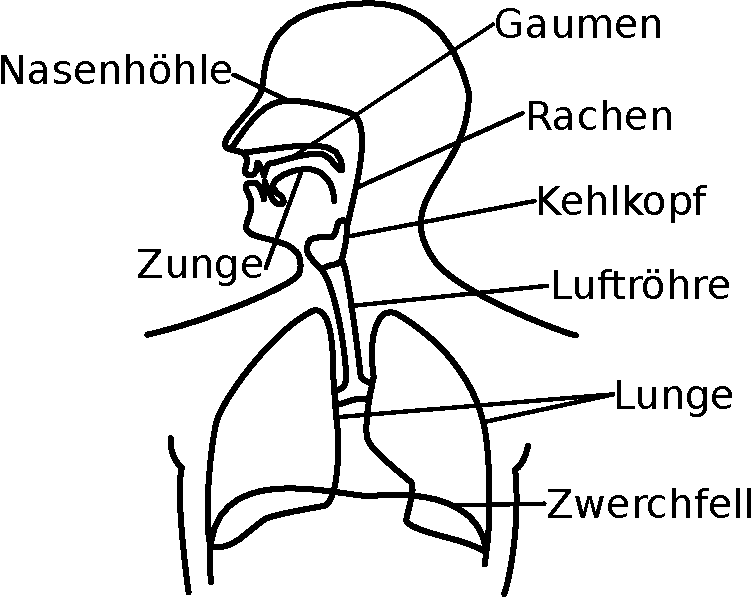
\includegraphics[width=6cm]{figures/ueberblick}
  \caption{Oberkörper und einige Organe}
  \label{fig:lunge}
\end{figure}

Das \textit{Zwerchfell} ist eine muskulöse Membran unterhalb der \textit{Lunge}, die den Herz- bzw.\ Lungenbereich von den Organen im Bauchraum trennt.
Durch Muskelanstrengung kann das Zwerchfell gesenkt werden, wodurch sich der Raum oberhalb vergrößert, wodurch wiederum ein Unterdruck relativ zur umgebenden Luft entsteht.
Durch diesen Unterdruck dehnt sich die Lunge aus, und weil sie durch die Luftröhre und den Mund- bzw.\ Nasenraum mit der umgebenden Luft verbunden ist, wird der Unterdruck mit einströmender Luft ausgeglichen (Einatmen).
Das Ausatmen ist ein passiver Vorgang, bei dem die Muskelanspannung des Zwerchfells gelöst wird, wodurch es in seine Ausgangsposition zurückkehrt und das Lungenvolumen verkleinert.
Der dabei entstehende Überdruck entweicht auf dem selben Weg, auf dem die Luft beim Einatmen eingeströmt ist.
Dieser Weg wird, wie schon erwähnt, überwiegend durch die gut zehn Zentimeter lange Luftröhre gebildet.

\TuBegin~Um diese Vorgänge nachzuvollziehen, können Sie sich direkt nach dem Ausatmen Nase und Mund zuhalten und versuchen, einzuatmen.
Sofort wird Ihnen die muskuläre Anspannung des Zwerchfells auffallen.
Außerdem wird bei zugehaltener Nase und zugehaltenem Mund das Gefühl des Unterdrucks im Brustkorb besonders auffallen, da keine Luft einströmen kann.

Dass wir diesen Luftstrom zum Sprechen benötigen, lässt sich auch leicht selber erfahren.
\TuBegin~Halten Sie die Luft an und versuchen dann, zu sprechen.
Es sollte Ihnen nicht gelingen.
Zur Kontrolle, dass Sie nicht doch atmen, hilft es, einen Spiegel dicht vor Mund und Nase zu halten.
Wenn Sie atmen, wird er beschlagen.

\subsection{Kehlkopf und Rachen}

\label{sec:kehlkopf}

Einfaches Ein- und Ausatmen verursacht zwar ein gewisses Rauschgeräusch, ist aber für viele Sprachlaute als grundlegender Mechanismus der Geräuschbildung nicht hinreichend.
Zu den vielen sprachlich relevanten Modifikationen des pulmonalen Luftstroms zählt die Benutzung des \textit{Kehlkopfes} (\textit{Larynx}).
Der Kehlkopf ist ein beweglich gelagertes System von Knorpeln.
Den vorderen, den sogenannten \textit{Schildknorpel}, kann man ertasten oder sogar sehen.
\TuBegin~Wenn Sie sich beim Sprechen vor einen Spiegel stellen oder an den Kehlkopf fassen, sehen bzw.\ merken Sie, wie er sich leicht auf und ab bewegt.

Die beiden sogenannten \textit{Stellknorpel} sind Teil des Kehlkopf-Systems.
Sie sind durch Muskelkraft kontrolliert bewegbar, und an ihnen sind die Stimmbänder aufgehängt.
Stellknorpel und Stimmbänder zusammen werden auch als die \textit{Glottis} bezeichnet.
Die relevante Funktion des Kehlkopfes aus Sicht der Phonetik ist die Produktion des \textit{Stimmtons}.
\TuBegin~Wenn Sie sich an den Kehlkopf/die Kehlkopfgegend fassen und verschiedene Wörter langsam sprechen (\zB \textit{Achat}, \textit{Verwaltungsangestellter}), werden Sie merken, dass der Kehlkopf bei einigen Segmenten (\textit{a}, \textit{w}, \textit{ng} usw.) eine Vibration produziert, bei anderen (\textit{ch}, \textit{t} usw.) aber nicht.

\index{Stimmton}
Diese Vibration ist der Stimmton.
Er entsteht dadurch, dass der pulmonale Luftstrom durch die Stimmlippen fließt, die dabei eine ganz bestimmte Spannung haben müssen.
Durch einen physikalischen Effekt (den \textit{Bernoulli-Effekt}) werden die Stimmlippen dabei dazu angeregt, in kürzesten Abständen (typischerweise mehrere hundert Mal pro Sekunde) aneinanderzuschlagen.
Diese Schläge erzeugen die charakteristische Vibration, die akustisch als Brummen oder Summen wahrgenommen wird und Sprachlaute als stimmhaft kennzeichnet.
In einem anderen, lockereren Spannungszustand vibrieren die Stimmlippen jedoch nicht, wenn Luft hindurchströmt.
\TuBegin~Sprechen Sie Wörter mit vielen \textit{h}-Segmenten am Silbenanfang aus, \zB \textit{Haha}, \textit{Hundehalter} usw.
Sie sollten bemerken dass beim \textit{h} im Kehlkopf zwar ein leichtes Rauschen entsteht, aber definitiv keinen Stimmton.

Als \textit{Rachen} (\textit{Pharynx}) bezeichnet man den Bereich zwischen Kehlkopf und Mundraum, der nach hinten durch eine relativ feste Wand begrenzt wird.
In Zusammenspiel mit der hinteren Zunge ist der Rachen in anderen Sprachen (\zB im Arabischen) an der Produktion von Segmenten beteiligt, im Standarddeutschen allerdings nicht.
\TuBegin~Ihren Rachen können Sie sehen, wenn Sie sich vor einen Spiegel stellen, die Zunge mit einem geeigneten Gegenstand herunterdrücken und \textit{ah} sagen.
Sie sehen dann geradeaus auf den oberen Rachenraum.

\subsection{Zunge, Mundraum und Nase}

\begin{figure}
  \centering
  \includegraphics[width=7cm]{figures/mundraum}
  \caption[Obere Sprechorgane und Artikulationsorte]{Obere Sprechorgane und Artikulationsorte}
  \label{fig:oberesprechorgane}
\end{figure}

Der Mundraum muss differenziert betrachtet werden, weil ein Großteil der Artikulation von Sprachlauten im Mundraum abläuft.
Eine wichtige Begrenzung des Mundraums nach unten ist die Zunge.
\TuBegin~Von Ihrer Zunge sehen Sie, wenn Sie sich vor den Spiegel stellen, nur den kleinsten Teil, nämlich den beweglichen Rücken und die bewegliche Spitze.
Der größte Teil der Zunge füllt den gesamten Bereich des Unterkiefers.
Auch hier gibt es die Möglichkeit, sich einen Eindruck davon zu verschaffen:
Fassen sie sich unter das Kinn (in den Bogen des Unterkiefers) und bewegen Sie die Zunge nach links und rechts.
Sie sollten spüren, wie sich größere muskuläre Strukturen bewegen.

Der bewegliche Teil der Zunge ist essentiell für die Bildung vieler Segmente.
Wenn wir den eigentlichen Mundraum von hinten nach vorne durchgehen, finden wir zunächst seine Begrenzung nach hinten: das \textit{Zäpfchen} (die \textit{Uvula}).
Am Zäpfchen werden tatsächlich Segmente des Deutschen gebildet, und zwar durch Anhebung des Zungenrückens.

Das \textit{Gaumensegel} (der \textit{weiche Gaumen}, das \textit{Velum}) ist ein weicher, mit Muskeln versorgter Abschnitt zwischen dem harten Gaumen und dem Zäpfchen.
\TuBegin~Man kann das Gaumensegel ertasten, indem man mit der Zunge oder einem Finger vorsichtig im Gaumen nach hinten fährt.
Während der vordere Gaumen hart ist, folgt weiter hinten eine weiche Stelle direkt vor dem Zäpfchen.
Den Zahndamm ertastet man auch sehr gut mit der Zungenspitze oder den Fingern.
Es handelt sich um die Stufe zwischen Zähnen und Gaumen.

Alle diese Teile der Mundhöhle spielen eine Rolle bei der Produktion standarddeutscher Segmente.
Eher eine indirekte Rolle bei der Sprachproduktion spielt die \textit{Nasenhöhle}.
\TuBegin~Halten Sie sich die Nase zu und sprechen Sie zunächst langanhaltend \textit{f} und \textit{s}, dann \textit{m} und \textit{n}.
Mit zugehaltener Nase sollte es nicht möglich sein, die \textit{m}- und \textit{n}-Segmente kontinuierlich auszusprechen.
Das liegt daran, dass bei diesen die Luft durch die Nasenhöhle statt durch die Mundhöhle abfließt.
Insofern ist die Nasenhöhle indirekt an der Produktion dieser Segmente beteiligt.

Zur weiteren Differenzierung des Gaumenbereichs spricht man bei der Stufe direkt hinter den Schneidezähnen vom \textit{Zahndamm} (die \textit{Alveolen}).
Außerdem sind \textit{Zähne} und \textit{Lippen} an der Sprachproduktion beteiligt, wobei hier davon ausgegangen wird, dass der Ort und die sonstige Funktion dieser Körperteile hinlänglich bekannt ist.

\section{Artikulationsart}

\label{sec:artikulationsart}

\subsection{Passiver und aktiver Artikulator}

\label{sec:artikulator}

Nachdem jetzt die an der Produktion deutscher Sprachlaute beteiligten Organe beschrieben wurden, müssen wir überlegen, wie diese Produktion genau abläuft.
Die Produktion des pulmonalen Luftstroms und des Stimmtons wurde schon beschrieben.
Im Grunde sind die einzigen Prinzipien der Produktion von Sprachlauten

\begin{enumerate}\Lf
  \item die \textit{Behinderung} (\textit{Obstruktion}) des Luftstroms, wodurch Geräusche (Zischen, Reiben, Knacken bzw.\ Knallen) entstehen, und
  \item die \textit{Veränderung von Resonanzen} der Mundhöhle durch Veränderung ihrer Form, was den Klang des Stimmtons verändert.
\end{enumerate}

Die Behinderung des Luftstroms findet an verschiedenen Stellen statt, und in diesem Zusammenhang sind zunächst die Begriffe \textit{aktiver und passiver Artikulator} zu erklären.
\TuBegin~Sprechen Sie langsam und sorgfältig das Wort \textit{Tante} und achten Sie darauf, wo sich die beweglichen Teile Ihres Mundraums jeweils befinden.
Sowohl die beiden \textit{t}-Segmente als auch die beiden \textit{n}-Segmente sind durch eine Berührung der Zunge an einer bestimmten Stelle innerhalb des Mundraums charakterisiert.
Versuchen Sie, die Stelle zu finden und anhand der Informationen aus Abschnitt~\ref{sec:anatomischegrundlagen} zu benennen, bevor Sie weiterlesen.

Beim \textit{t} und beim \textit{n} legt sich die vordere Zungenspitze gegen den Zahndamm.
Die Zunge ist dabei beweglich, der Zahndamm hingegen unbeweglich.
Dass sich zwei Körperteile auf diese Weise berühren bzw.\ annähern, ist charakteristisch für viele Artikulationen, und man nennt sie daher die \textit{Artikulatoren}.

\Definition{Artikulator}{
\label{def:artikulator}
Ein Artikulator ist ein Körperteil, der an einer Artikulation beteiligt ist.
Ein aktiver Artikulator führt dabei eine Bewegung zu einem sich nicht bewegenden passiven Artikulator aus.
\index{Artikulator}
}

Was die Artikulatoren bei welchen Segmenten genau machen, wird \textit{Artiulationsart} genannt und in den folgenden Abschnitten klassifiziert und illustriert.

\Definition{Artikulationsart}{\label{def:artart} Die Artikulationsart eines Segmentes ist die Art und Weise, in der der Luftstrom aus der Lunge durch die Artikulatoren behindert wird.}

\subsection{Stimmhaftigkeit}

\label{sec:stimmhaftigkeit}

Zunächst können wir eine grundlegende Unterscheidung in der Artikulationsart vornehmen.
In \ref{sec:kehlkopf} wurde bereits beschrieben, dass manche Segmente mit Stimmton produziert werden, aber andere nicht.
Man kann also Segmente nach ihrer \textit{Stimmhaftigkeit} unterscheiden.

\Definition{Stimmhaftigkeit}{
Ein Segment ist stimmhaft, wenn zeitgleich zu seiner primären Artikulation ein Stimmton produziert wird.
\index{Stimmhaftigkeit}
}

\subsection{Obstruenten}

Bei der zuerst zu besprechenden Gruppe von Segmenten handelt es sich um die sogenannten \textit{Obstruenten} (\textit{Geräuschlaute}, wörtlich im Latein eigentlich \textit{Hindernislaute}).
Nach der Definition folgen Abschnitte über die Unterarten von Obstruenten.

\Definition{Obstruent}{
Ein Obstruent ist ein Segment, bei dem der pulmonale Luftstrom durch eine Verengung, die die Artikulatoren herstellen, am freien Abfließen gehindert wird.
Es entstehen Geräuschlaute:
Entweder Knall- bzw.\ Knack-Laute oder Reibegeräusche durch Turbulenzen im Luftstrom.
\index{Obstruent}
}

\subsubsection{Plosive}

Bei \textit{k}-, \textit{t}- und \textit{p}-Segmenten (ähnlich \textit{g}, \textit{d}, \textit{b}) wird der Luftstrom jeweils kurz unterbrochen, und nach der Unterbrechung folgt ein deutlicher Schwall von Luft, der dann wieder abebbt.
Das liegt daran, dass die Artikulatoren einen vollständigen Verschluss des Mundraumes herstellen, der dann spontan gelöst wird.
Das entstehende Geräusch ähnelt einem Knall, und die betreffenden Segmente heißen \textit{Plosive}.
\TuBegin~Halten Sie sich eine Handfläche dicht vor den Mund und sprechen Sie folgende Wörter sorgfältig aus: \textit{Kuckuck}, \textit{Torte}, \textit{Pappe}.
Es fällt sofort auf, dass der Luftstrom nicht gleichmäßig (wie beim einfachen Atmen) aus dem Mund entweicht.

\Definition{Plosiv}{
Ein Plosiv ist ein Obstruent, bei dem einer totalen Verschlussphase eine Lösung des Verschlusses folgt und ein Knall- oder Knackgeräusch entsteht.
\index{Plosiv}
}

Plosive können wie bereits erwähnt nach Stimmhaftigkeit unterschieden werden, wie an den Wörtern \textit{danke}/\textit{tanke}, \textit{banne}/\textit{Panne}, \textit{Gabel}/\textit{Kabel} demonstriert werden kann.
Hier entsprechen jeweils \textit{d} und \textit{t}, \textit{b} und \textit{p} sowie \textit{g} und \textit{k} einem stimmhaften und einem stimmlosen Segment.

\subsubsection{Frikative}

Das Geräusch, das bei \textit{Frikativen} entsteht, kann als Rauschen (oder Reibegeräusch) beschrieben werden.
Daher kommt auch der Name, der mit \textit{Reibelaute} eingedeutscht werden kann.
\TuBegin~Sprechen und fühlen Sie folgende Wörter: \textit{Skischuhe}, \textit{Fach}, \textit{Wicht}.
Bei den Segmenten, die durch \textit{sch} (und in \textit{Ski} ausnahmsweise \textit{sk}), \textit{f}, \textit{ch} und \textit{w} wiedergegeben werden, spüren Sie ein konstantes, mehr oder weniger scharfes Entweichen von Luft.

\Definition{Frikativ}{
Ein Frikativ ist ein Obstruent, bei dem durch die Artikulatoren ein vergleichsweise enge aber nicht vollständige Verengung im Weg des pulmonalen Luftstroms hergestellt wird, wodurch dieser stark verwirbelt wird (Turbulenzen) und ein rauschendes Geräusch erzeugt wird.
\index{Frikativ}
}

Bemerkenswert ist außerdem, dass die Frikative (im Gegensatz zu den Plosiven) so lange artikuliert werden können, wie der Luftstrom aufrecht erhalten werden kann.
Die Segmente sind also \textit{kontinuierlicher} als Plosive.
Auch unter den Frikativen gibt es stimmlose und stimmhafte: \textit{sch}, \textit{ch} und \textit{f} sind stimmlos, \textit{w}-Laute aber \zB stimmhaft.
Auch das \textit{j}-Segment (\textit{Jahr}) wird oft als Frikativ artikuliert.

\subsubsection{Affrikaten}

\textit{Affrikaten} sind komplexe Segmente, nämlich eine direkte Abfolge von einem Plosiv und einem Frikativ.
Beispiele sind das \textit{ts}-Segment (orthographisch \textit{z}) in Wörtern wie \textit{Zuschauer} oder das \textit{pf}-Segment wie in \textit{Pfund}.

\Definition{Affrikate}{
\label{def:affrikate}
Eine Affrikate ist ein komplexer Obstruent aus einem Plosiv und einem folgenden Frikativ.
Der beteiligte Plosiv und der beteiligte Frikativ sind dabei \textit{homorgan} (an derselben Stelle gebildet).
\index{Affrikate}
}

Die deutschen \textit{pf}-Segmente sind \zB streng genommen nicht homorgan, wie in Abschnitt~\ref{sec:affrikatenhomorgan} diskutiert wird.
Die Frage, ob wirklich eine Affrikate oder doch zwei Segmente vorliegen, ist oft nur schwer zu entscheiden und manchmal eher eine Frage der Phonologie als der Phonetik.

\subsection{Laterale Approximanten}

Im Deutschen ist das \textit{l}-Segment der einzige \textit{laterale Approximant}.
Dabei wird die Zungenspitze mittig an den Zahndamm gelegt, seitlich der Zunge fließt der Luftstrom aber ungehindert ab.
\TuBegin~Beobachten Sie (möglichst vor dem Spiegel), wie im Wort \textit{Ball} das letzte Segment gebildet wird.

\Definition{Lateraler Approximant}{
Ein lateraler Approximant ist ein Segment, bei dem neben einem zentralen Verschluss der Artikulatoren der Luftstrom weitgehend ungehindert ohne Bildung von Turbulenzen abfließt.
\index{Approximant}
}

\subsection{Nasale}

Wir haben bereits den Test gemacht, Wörter mit \textit{n} und \textit{m} mit zugehaltener Nase auszusprechen, und dabei festgestellt, dass dies unmöglich ist.
Bei diesen beiden Segmenten handelt es sich um \textit{Nasale}.
Bei Nasalen wird der Mundraum vollständig verschlossen, die Luft kann nirgendwohin entweichen, und die Artikulation wird unmöglich.
Dass wir verschiedene nasale Obstruenten akustisch voneinander unterscheiden können, liegt wieder an unterschiedlichen Resonanzen, genauso wie bei den Approximanten und den Vokalen (s.\ Abschnitt~\ref{sec:vokale}).

\Definition{Nasal}{
Ein Nasal ist ein Segment, bei dem durch einen vollständigen Verschluss im Mundraum (und eine Absenkung des Velums) die Luft zum Entweichen durch die Nasenhöhle gezwungen wird.
Es entstehen keine Turbulenzen.
\index{Nasal}
}

\subsection{Vokale}

\label{sec:vokale}

\textit{Vokale} werden in der Schulgrammatik gerne als \textit{Selbstlaute} bezeichnet und damit den Konsonanten als \textit{Mitlauten} gegenübergestellt.
Die Idee hinter dieser Bezeichnung ist, dass die Vokale selbständig (also für sich allein) ausgesprochen werden können, wohingegen die Konsonanten nur mit einem anderen Segment (einem Vokal) zusammen ausgesprochen werden können.
Diese Einordnung ist grundlegend falsch, da alle Konsonanten (ggf.\ nach entsprechendem phonetischen Training) selbständig realisiert werden können.
Bei Frikativen und nasalen Obstruenten ist sogar die kontinuierliche Artikulation möglich.
Da wir einen intuitiven Begriff von Vokalen haben und die orthographisch als \textit{a}, \textit{e}, \textit{i}, \textit{o}, \textit{u} sowie \textit{ä}, \textit{ö}, \textit{ü} wiedergegebenen Segmente als Vokale bereits kennen, können wir überlegen, was das Besondere an ihnen ist.
\TuBegin~Sprechen Sie sich die Vokalsegmente vor und beobachten Sie dabei (einschließlich Beobachtung im Spiegel), wie sich die Zunge, die Lippen und die sonstigen Organe im Mundraum dabei verhalten. Wenn Sie bei der Produktion von Vokalen wieder Ihren Kehlkopf ertasten, werden Sie außerdem feststellen, dass alle stimmhaft sind.

Die Zunge bewegt sich bei der Artikulation verschiedener Vokale im Mund\-raum zu verschiedenen Positionen, aber es findet bei keinem der Segmente eine deutliche Verengung an irgendeinem Artikulator statt.
Der Luftstrom kann daher weitgehend ungehindert abfließen.
Außerdem verändert sich die Formung der Lippen von rund (\zB bei \textit{u}) zu eher breit (\zB bei \textit{e}).

\Definition{Vokal}{
\label{def:vokal}
Ein Vokal ist ein Segment, bei dem der pulmonale Luftstrom weitgehend ungehindert abfließen kann, und bei dem keine geräuschhaften Anteile entstehen.
Der Klang eines Vokals wird durch eine spezifische Formung des Resonanzraumes erzeugt.
\index{Vokal}
}

Man muss an dieser Stelle wenigstens intuitiv definieren, was Resonanzen sind.
Das Phänomen, dass physikalische Körper abhängig von ihrer Form und ihrem Material einen Klang verändern, der in ihnen produziert wird, lässt sich leicht nachvollziehen.
Wenn man in ein Rohr aus Holz, in ein Metallrohr, in die hohle Hand oder in einen hohlen Betonklotz einen Ton singt, klingt dieser jeweils unterschiedlich.
Das liegt daran, dass ein Körper abhängig von seinem Material, seiner Form und Größe bestimmte Frequenzen eines Klangs verstärkt und abschwächt.
Körper haben also ein charakteristisches \textit{Resonanzverhalten} abhängig von Form und Material.
Das Resonanzverhalten des Mundraums wird nun bei Vokalen gezielt durch die Positionierung der Zunge und der Lippen verändert, denn durch die Positionierung dieser Artikulatoren ändert sich die Form des Mundraums.
Wir können also \textit{a} und \textit{i} voneinander unterscheiden, weil das Ausgangssignal des Stimmtons bei diesen Segmenten jeweils mit einem unterschiedlich geformten Mundraum zu einem anderen Klang geformt wird.

\subsection{Oberklassen für bestimmte Artikulationsarten}

\label{sec:photoberklassen}

Bei den Vokalen, Approximanten und Nasalen enthielten die Definitionen jeweils das Kriterium, dass keine Turbulenzen entstehen, während der Luftstrom abfließt.
Außerdem gibt es natürlich bei diesen Segmenten keine spontane Verschlusslösung mit Knallgeräusch wie bei den Plosiven.
Daher gibt es hier den Oberbegriff des \textit{Sonoranten}, der diese Segmente zusammenfasst und den Obstruenten gegenüberstellt.
Typisch, aber nicht notwendig für die Sonoranten ist die Stimmhaftigkeit.

\Definition{Sonoranten und Obstruenten}{
Sonoranten (Klanglaute) sind nicht-geräuschhafte Segmente, bei denen der pulmonale Luftstrom ohne Bildung von Turbulenzen durch den Mund oder die Nase abfließen kann.
Alle anderen Segmente gelten als geräuschhaft und werden Obstruenten (Geräuschlaute) genannt.
\index{Sonorant}
\index{Obstruent}
}

\Satz{Sonoranten und Stimmton}{
Sonoranten sind prototypisch stimmhaft.
}

Die Unterscheidung von Vokalen und Konsonanten hat nichts mit der Unterscheidung von Sonoranten und Obstruenten zu tun.
Die Konsonanten sind eine Sammelklasse für alle Sonoranten und Obstruenten, die keine Vokale sind.

\Definition{Konsonanten}{
Konsonanten sind alle Obstruenten, Approximanten und Nasale.
Es sind die Segmente, die typischerweise (aber nicht notwendigerweise) nicht silbisch sind, also prototypischerweise alleine keine Silbe bilden können.
\index{Konsonant}
}

Damit ergibt sich das Diagramm in \ref{fig:lautklassen} für die Klassifizierung der Segmente in der Phonetik.
In Abschnitt~\ref{sec:photpholmerkmale} werden weitere Gründe diskutiert, warum diese Klassifizierung wichtig ist.

\begin{figure}
  \centering
  \Treek[2.5]{4}{
    & \K{\textbf{Sonoranten}}\Below{(Klanglaute)}\BBel{dl}\BBel{d}\BBel{dr} &&& \K{\textbf{Obstruenten}}\Below{(Geräuschlaute)}\BBel{dl}\BBel{d}\BBel{dr} \\
    \K{\textbf{Vokale}}\Below{(silbisch)} & \K{Approximanten}\B{drr} & \K{Nasale}\B{dr} & \K{Plosive}\B{d} & \K{Frikative}\B{dl} & \K{Affrikaten}\B{dll} \\
    &&& \K{\textbf{Konsonanten}}\Below{(nicht silbisch)} \\
  }
  \caption{Grobe Klassifikation der Segmente in der Phonetik}
  \label{fig:lautklassen}
\end{figure}

\section{Artikulationsort}

\label{sec:artort}

Bisher haben wir uns darauf beschränkt, festzustellen, auf welche Art bestimmte Segmente gebildet werden.
In einigen Fällen (\zB beim \textit{l}-Segment) haben wir auch schon festgestellt, wo die Artikulatoren ggf.\ einen Verschluss oder eine Annäherung herstellen, aber das muss noch systematisch geschehen.
Dabei leitet uns Definition~\ref{def:artort}.
Gleichzeitig werden die für die Transkription des Deutschen benötigten Zeichen des weitest verbreiteten phonetischen Alphabets vorgestellt.

\Definition{Artikulationsort}{\label{def:artort} Der Artikulationsort eines Segments ist der Punkt der größten Annäherung zwischen den Artikulatoren.}

\subsection{IPA:\ Grundzeichen und Diakritika}

\index{IPA}

Das übliche phonetische Alphabet ist das der \textit{International Phonetic Association} (IPA).%
\footnote{\url{https://www.internationalphoneticassociation.org/}}	
Es basiert auf der Lateinschrift und stellt für alle in menschlichen Sprachen vorkommenden Segmente eine mögliche Schreibung zur Verfügung.
Dabei werden primäre Artikulationen in der Regel durch ein Buchstabensymbol dargestellt.
Hinzu kommen sog.\ Diakritika (Zusatzzeichen), die vor, über, unter oder neben dem Hauptzeichen geschrieben werden und genauere Informationen zur primären Artikulation kodieren.
Hier besteht also tatsächlich der Anspruch, ein System vorzulegen, in dem man so schreibt, wie man spricht (vgl.\ Abschnitt~\ref{sec:unphonetischeschreibungen}).

Es ist üblich, phonetische Transkriptionen in [~] zu schreiben, und wir übernehmen hier diese Konvention.
Man unterscheidet gemeinhin eine enge Transkription von einer weiten oder lockeren Transkription.
Bei einer engen Transkription versucht man, jedes artikulatorische Detail, das man hört, genau festzuhalten, auch die linguistisch vielleicht irrelevanten.
Bei der lockeren Transkription geht es nur darum, die wichtigen Merkmale der gehörten Segmente aufzuschreiben.
Die lockere Transkription ist prinzipiell problematisch, weil sie dazu tendiert, zu viel phonologisches Wissen in die Transkription einzubeziehen.
Eine phonetische Transkription sollte im Normalfall so beschaffen sein, dass sie genau wiedergibt, was man tatsächlich gehört hat.
Da es hier aber nur um einen ersten Einblick geht, ist unsere Transkription nicht übermäßig genau, möglichst ohne dass sich dabei verfälschende Vereinfachungen einschleichen.

\subsection{Laryngale bzw.\ Glottale}

\label{sec:photlaryngale}

\index{Laryngal}

Im Bereich des Kehlkopfs (Larynx) bzw.\ des Stimmlippensystems (Glottis) bilden Sprecher des Standarddeutschen nur zwei Segmente.%
\footnote{Für normale phonetische Belange ist die Unterscheidung von Glottis und Larynx nicht relevant, und man findet sowohl die Bezeichnung \textit{glottal} als auch \textit{laryngal}.}
Der eine ist der stimmlose laryngale Frikativ \textipa{[h]}.
In Wörtern wie \textit{Hoffenheim}, \textit{Handspiel} usw.\ kommt dieses Segment am Anfang vor.
Weiterhin ist der stimmlose laryngale Plosiv \textipa{[P]} sehr charakteristisch für das Deutsche.
\TuBegin~Wenn Sie Wörter wie \textit{Anpfiff} oder \textit{energisch} sehr deutlich und energisch aussprechen, hören Sie am Anfang des Wortes einen Plosiv, einen Knacklaut im Kehlkopf.
Er tritt auch vor dem \textit{o} in \textit{Chaot} (nicht aber in \textit{Chaos}), vor dem \textit{ei} in \textit{Verein} oder vor dem \textit{äu} in \textit{beäugen} auf.

Bei diesem bilden die Stimmlippen als aktive Artikulatoren einen Verschluss, der spontan gelöst wird.
Wenn wir das IPA-Zeichen \textipa{P} vorläufig in die normale Orthographie einfügen, ergibt sich für die obigen Wörter (\ref{ex:phot2529}).

\begin{exe}
  \ex\label{ex:phot2529}
  \begin{xlist}
    \ex{\textipa{P}Anpfiff}
    \ex{\textipa{P}energisch}
    \ex{Cha\textipa{P}ot}
    \ex{Chaos, \Ast Cha\textipa{P}os}
    \ex{Ver\textipa{P}ein}
    \ex{be\textipa{P}äugen}
  \end{xlist}
\end{exe}

Dieser laryngale Plosiv (auch \textit{Glottalverschluss}, \textit{Glottisverschluss} oder englisch \textit{glottal stop}) tritt regelhaft vor jedem vokalisch anlautenden Wort und auch vor jeder vokalisch anlautenden betonten Silbe innerhalb eines Wortes auf.
Zur Wortbetonung (dem Akzent) wird erst in Abschnitt~\ref{sec:prosodie} Substantielles gesagt.
Dort wird die Regel für die \textipa{[P]}-Einfügung weiter motiviert und illustriert.
Viele Sprachen haben einen vokalischen Anlaut ohne diesen Plosiv.
Er ist daher typisch für einen deutschen Akzent in vielen Fremdsprachen, der oft als abgehackt wahrgenommen wird.
Umgekehrt ist sein Fehlen verantwortlich dafür, dass fremdsprachliche Akzente im Deutschen von Erstsprechern des Deutschen oft als konturlos o.\,ä.\ wahrgenommen werden.

\subsection{Uvulare}

\index{Uvular}

Am Zäpfchen werden der stimmlose und der stimmhafte uvulare Frikativ gebildet: \textipa{[X]} und \textipa{[K]}.
Der stimmlose wird \textit{ch} geschrieben und tritt nur nach bestimmten Vokalen auf, also in Wörtern wie \textit{ach}, \textit{Bach}, \textit{Tuch}.%
\footnote{Die oft zu findende Behauptung, in Wörtern wie \textit{Buch} handele es sich im deutschen Standard um einen am weichen Gaumen artikulierten Velar \textipa{[x]} (s.\ Abschnitt~\ref{sec:velar}) kann ich nicht nachvollziehen.
Außer evtl.\ in Dialekten wie dem Sauerländischen findet die Artikulation gut hörbar weiter hinten im Mundraum statt, also am Zäpfchen.
}
Der stimmhafte kommt nicht bei allen Sprechern des Deutschen vor, ist aber die häufigste phonetische Realisierung von \textit{r} im Silbenanlaut, also in \textit{rot}, \textit{berauschen} usw.
\TuBegin~Zur bewussten Lokalisierung von \textipa{[X]} und \textipa{[K]}, die im hinteren Bereich der Mundhöhle gebildet werden, hilft es, die vordere Zunge mit einem geeigneten Gegenstand herunterzudrücken und dann \zB \textit{Rache} zu sagen (mit \textipa{[K]} und \textipa{[X]}).
Das klingt zwar wegen der eingeschränkten Artikulation der Vokale etwas ungewöhnlich, die Konsonanten können aber einwandfrei realisiert werden.
Hier ist zwar die Zunge der aktive Artikulator, aber nur mit dem hinteren Teil, dem Zungenrücken.

\subsection{Velare}

\label{sec:velar}

\index{Velar}

Das Velum oder Gaumensegel ist einer von mehreren Artikulationsorten, an denen im Deutschen ein stimmloser und ein stimmhafter Plosiv sowie ein Nasal artikuliert werden.
\TuBegin~Halten Sie wieder die Zungenspitze fest und artikulieren Sie \textit{King Kong} und \textit{Gang}.
Die Artikulation sollte ähnlich gut gelingen wie bei \textit{Rache}, weil auch hier die Zungenspitze nicht beteiligt ist.
Mit ein bisschen Mühe ist es möglich, den Ort und die Art der Artikulation dieser Segmente im Selbstversuch auch visuell zu beobachten.
Dazu stellt man sich vor einen Spiegel und lässt den Mund so weit wie möglich geöffnet bei der Artikulation der Beispielwörter.
Man kann dann sehen, wie sich der Zungenrücken an das Gaumensegel hebt, und wie ggf.\ der Verschluss gelöst wird.

Die \textit{k}-, \textit{g}- und \textit{ng}-Segmente werden also alle im hinteren Mundraum artikuliert, und zwar am Velum.
Der Zungenrücken ist dabei der aktive Artikulator.
Die IPA-Schreibungen sind sehr transparent: \textipa{[k]}, \textipa{[g]} und \textipa{[N]}.
Zu beachten ist, dass orthographisches \textit{ng} zumindest in der Phonetik einem Laut und nicht etwa zwei Lauten entspricht.

\subsection{Palatale}

\index{Palatal}

Am harten Gaumen finden wir im Deutschen nur das \textit{j}-Segment wie in \textit{Jahr}, \textit{Jugend} usw. und den so genannten \textit{ich}-Laut.
Das \textit{j}-Segment wird meist als palataler stimmhafter Frikativ \textipa{[J]} realisiert.
Der \textit{ich}-Laut hingegen ist immer ein palataler stimmloser Frikativ \textipa{[\c{c}]}.

\subsection{Palato-Alveolare und Alveolare}

\index{Alveolar}

Am Übergang vom harten Gaumen zum Zahndamm und am Zahndamm finden sich eine ganze Reihe von Segmenten in verschiedenen Artikulationsarten, sowohl stimmlos als auch stimmhaft.
\TuBegin~Sprechen Sie die folgenden Wörter und achten Sie auf die Anlaute: \textit{lang}, \textit{schön}, \textit{Tor}, \textit{Didi}.
Diese Segmente werden am unteren Teil des Zahndamms gebildet.
Wenn Sie in diesem Fall die Zungenspitze festhalten, können Sie diese Wörter nicht auf verständliche Weise aussprechen.

Die hier besprochenen Segmente werden im Gegensatz zu den Uvularen und Velaren mit der Zungenspitze als aktivem Artikulator gebildet.
Das \textit{l}-Segment ist der palato-alveolare laterale Approximant und wird \textipa{[l]} transkribiert.
Das \textit{sch}-Segment, bei dem meistens zusätzlich die Lippen rund geformt werden, wird \textipa{[S]} transkribiert.
Zusätzlich gibt es noch den stimmhaften palato-alveolaren Frikativ \textipa{[Z]} wie in \textit{Garage}, \textit{Marge} oder anderen, meist französischen Lehnwörtern.
Weil diese Wörter nicht zum Kernwortschatz gehören (s.\ Abschnitt~\ref{sec:kern}), lassen wir \textipa{[Z]} im weiteren Verlauf aus Übersichtstabellen usw.\ heraus.
Etwas weiter vorne werden die Anlaute folgender Wörter gesprochen, ebenfalls mit der Zungenspitze als aktivem Artikulator: \textit{Tor}, \textit{dort}, \textit{neu}, \textit{Sahne}.
Gleiches gilt für das letzte Segment in folgendem Wort: \textit{Schluss}.
Wir haben hier eine komplette Reihe von alveolarem stimmlosen Plosiv \textipa{[t]}, alveolarem stimmhaften Plosiv \textipa{[d]}, alveolarem Nasal \textipa{[n]}, alveolarem stimmhaften Frikativ \textipa{[z]} (wie in \textit{Sahne}) und alveolarem stimmlosen Frikativ \textipa{[s]} wie in \textit{Schluss}.%
\footnote{Die Segmente \textipa{[s]} und \textipa{[z]} werden dabei eigentlich etwas weiter vorne in Richtung der Zähne artikuliert.}

\subsection{Labiodentale und Bilabiale}

\index{Labial}

Im Bereich der Konsonanten sind wir von unten nach oben und hinten nach vorne durch den Vokaltrakt vorgegangen und erreichen jetzt den Bereich der Lippen.
\TuBegin~Vor dem Spiegel sieht man gleich, dass Wörter wie \textit{Pass} oder \textit{Ball} mit einem an der gleichen Stelle artikulierten Segment beginnen.
Beide Lippen (als aktive Artikulatoren) schließen sich und lösen daraufhin den Verschluss.
Es handelt sich um den stimmlosen bilabialen Plosiv \textipa{[p]} und den stimmhaften bilabialen Plosiv \textipa{[b]}.

Während bei den zuletzt genannten Segmenten beide Lippen beteiligt sind (daher der Terminus \textit{bilabial}), erkennt man bei den Anlauten von \textit{Fuß} und \textit{Wade}, dass die Zähne des Oberkiefers beteiligt sind, die sich an die Unterlippe legen.
Dort erzeugen sie keinen Verschluss sondern eine Verengung mit Reibegeräusch.
Es handelt sich daher um den stimmlosen und den stimmhaften \textit{labio-dentalen} Frikativ (\textipa{[f]} und \textipa{[v]}).

\subsection{Affrikaten und Artikulationsorte}

\label{sec:affrikatenhomorgan}

\index{Affrikate!Homorganität}

In den Wörtern \textit{Dschungel}, \textit{Chips}, \textit{Zange}, \textit{Pfanne} finden wir anlautend das gesamte Inventar der phonetischen Affrikaten im Deutschen.
Diese bestehen aus zwei aufeinanderfolgenden Phasen: einer plosiven Phase und einer frikativen Phase.
Man schreibt im IPA-Alphabet daher diese Segmente mit den Grundzeichen für den Plosiv und den Frikativ mit einem verbindenden Bogen (der \textit{Ligatur}).
Für die stimmlose palato-alveolare Affrikate wie in \textit{Matsch} schreibt man \textipa{[\t{tS}]}, für die stimmlose alveolare Affrikate wie in \textit{Zange} \textipa{[\t{ts}]} und für die stimmlose labiale Affrikate wie in \textit{Pfanne} \textipa{[\t{pf}]}.
Nur in Lehnwörtertn findet man die stimmhafte palato-alveolare Affrikate wie in \textit{Dschungel}, transkribiert \textipa{[\t{dZ}]}.

Wenn wir uns \textipa{[\t{pf}]} ansehen, stellen wir fest, dass die Bedingung der Homorganität aus Definition~\ref{def:affrikate} (S.~\pageref{def:affrikate}) strenggenommen nicht erfüllt wird, denn \textipa{[p]} ist bilabial und \textipa{[f]} labio-dental.
Insofern werden die beiden Teile der Affrikate zwar ziemlich nah beieinander gebildet, aber nicht wirklich am selben Ort.
Ohne uns in die Details dieses Problems zu vertiefen, stellen wir dies hier fest, behandeln \textipa{[\t{pf}]} aber im weiteren Verlauf als Affrikate.

\begin{table}
  \centering
  \begin{tabular}{rccccccccc}
    \lsptoprule
    \multicolumn{1}{c}{} & \Sw{\textbf{bilabial}} & \Sw{\textbf{labio-dental}} & \Sw{\textbf{alveolar}} & \Sw{\textbf{palato-alveolar}} & \Sw{\textbf{palatal}} & \Sw{\textbf{velar}} & \Sw{\textbf{uvular}} & \Sw{\textbf{laryngal}} \\
    \midrule
    \textbf{stl.\ Plosiv} & \textipa{p} & \textipa{} & \textipa{t} & \textipa{} & \textipa{} & \textipa{k} & \textipa{} & \textipa{P} \\
    \textbf{sth.\ Plosiv} & \textipa{b} & \textipa{} & \textipa{d} & \textipa{} & \textipa{} & \textipa{g} & \textipa{} & \textipa{} \\
    \textbf{stl.\ Frikativ} & \textipa{} & \textipa{f} & \textipa{s} & \textipa{S} & \textipa{\c{c}} & \textipa{} & \textipa{X} & \textipa{h} \\
    \textbf{sth.\ Frikativ} & \textipa{} & \textipa{v} & \textipa{z} & \textipa{} & \textipa{J} & \textipa{} & \textipa{K} & \textipa{} \\
    \textbf{stl.\ Affrikate} & \textipa{} & \textipa{\t{pf}} & \textipa{\t{ts}} & \textipa{\t{tS}} & \textipa{} & \textipa{} & \textipa{} & \textipa{} \\
    \textbf{sth.\ Affrikate} & \textipa{} & \textipa{} & \textipa{} & \textipa{} & \textipa{} & \textipa{} & \textipa{} & \textipa{} \\
    \textbf{lateraler Approximant} & \textipa{} & \textipa{} & \textipa{} & \textipa{l} & \textipa{} & \textipa{} & \textipa{} & \textipa{} \\
    \textbf{Nasal} & \textipa{m} & \textipa{} & \textipa{n} & \textipa{} & \textipa{} & \textipa{N} & \textipa{} & \textipa{} \\
    \lspbottomrule
  \end{tabular}
  \caption{IPA:\ Konsonanten des Deutschen}
  \label{tab:photkons}
\end{table}

\subsection{Vokale und Diphthonge}

\subsubsection{Vokale}

\index{Vokal}

Für die phonetische Klassifikation der Vokale werden in diesem Abschnitt \textit{Höhe} und \textit{Lage} als eine Art vokalischer Artikulationsort eingeführt.
Außerdem werden \textit{Rundung} und \textit{Länge} diskutiert, die strenggenommen nicht zum Artikulationsort gehören.%
\footnote{Die IPA-Symbole sind nun nahezu vollständig eingeführt und alle Beispielwörter werden ab jetzt vollständig transkribiert.}
Man fasst die Vokale normalerweise in einem sogenannten \textit{Vokalviereck} (manchmal auch \textit{Vokaltrapez} genannt) zusammen, s.\ Tabelle~\ref{tab:vokaltrap}.
Das Vokalviereck ist nichts anderes als eine Tabelle, in der die Spalten die Lage und die Zeilen die Höhe kodieren.
Wenn es eine ungerundete und eine gerundete Variante gibt, steht die gerundete stets an zweiter Stelle.
Länge wird hier nicht verzeichnet.
Der Rest dieses Abschnitts erläutert das Vokalviereck im Detail.

\index{Vokalviereck}

\begin{table}
  \centering
  \begin{tabular}{cccccc}
    \lsptoprule
    \multicolumn{1}{c}{} && \textbf{halb-} && \textbf{halb-} & \\
    \multicolumn{1}{c}{} & \textbf{vorne} & \textbf{vorne} & \textbf{zentral} & \textbf{hinten} & \textbf{hinten} \\
    \midrule
    \textbf{hoch/geschlossen} & \textipa{i y} &&&& \textipa{u} \\
    \multirow{2}{*}{\textbf{halbhoch}} && \textipa{I Y} && \textipa{U} & \\
    & \textipa{e} \textipa{\o} &&&& \textipa{o} \\
    \textbf{mittel} &&& \textipa{@} && \\
    \multirow{2}{*}{\textbf{halbtief}}& \textipa{E} \textipa{\oe} &&&& \textipa{O} \\
    &&& \textipa{5} && \\
    \textbf{tief/offen} &&& \textipa{a} && \\
    \lspbottomrule
  \end{tabular}
  \caption{IPA-Vokalviereck für das Deutsche}
  \label{tab:vokaltrap}
\end{table}

Vokale sind gewöhnlicherweise bezüglich ihres Artikulationsorts schwerer einzuordnen als Konsonanten.
Dies liegt daran, dass es für Vokale keinen gut lokalisierbaren punktuellen Artikulationsort gibt und die Orientierung im Mundraum dadurch erschwert wird.
Vielmehr wird die Zunge (sehr vereinfacht gesprochen) höher oder tiefer und weiter vorne oder weiter hinten im Mundraum lokalisiert.
Entsprechend unterscheidet man Vokale nach ihrer \textit{Lage} als \textit{vorne}, \textit{zentral} oder \textit{hinten} und ihrer \textit{Höhe} als \textit{hoch}, \textit{mittel} oder \textit{tief}.
Wenn Zwischenstufen benötigt werden, heißen diese \textit{halbvorne}, \textit{halbhinten} und \textit{halbhoch}, \textit{halbtief}.
Somit hat man auf beiden Achsen eine fünffache Unterscheidung, die insbesondere in der Phonologie ggf.\ durch elegantere Formulierungen reduziert werden kann.
Hohe Vokale kommen beispielsweise in \textit{lieb} \textipa{[li:p]}, \textit{lüg} \textipa{[ly:k]}, \textit{Trug} \textipa{[tKu:k]} vor, wobei \textipa{[i]} und \textipa{[y]} vorne liegen und \textipa{[u]} hinten.
Der tiefste Vokal ist \textipa{[a]} wie in \textit{Lab} \textipa{[la:p]}.

\index{Lippenrundung}
Weiterhin werden Vokale nach \textit{Lippenrundung} weiter unterschieden.
Der einzige Unterschied zwischen \textipa{[i]} in \textit{Liege} \textipa{[li:g@]} und \textipa{[y]} in \textit{Lüge} \textipa{[ly:g@]} oder \textipa{[e]} in \textit{Wege} \textipa{[ve:g@]} und \textipa{[\o]} in \textit{wöge} \textipa{[v\o:g@]} ist also der der Rundung.
\TuBegin~Wenn Sie wieder ein Spiegel-Experiment machen und zunächst \textit{u}, \textit{o}, \textit{ü} und \textit{ö} sprechen und dann \textit{a}, \textit{i}, \textit{e} und \textit{ä}, dann werden Sie beobachten, dass bei der Artikulation der ersten Gruppe die Lippen gerundet sind, bei der zweiten Gruppe aber nicht.

Die \textit{Länge} bezieht sich schließlich auf die Zeitdauer, für die ein Segment artikuliert wird.
Das ist nicht absolut zu verstehen, in dem Sinn, dass lange und kurze Vokal eine bestimmte Zeit von Millisekunden dauern, sondern relativ zueinander.
Es gibt von bestimmten Vokalen -- nämlich \textipa{[i]}, \textipa{[y]}, \textipa{[u]}, \textipa{[e]}, \textipa{[\o]}, \textipa{[o]} und \textipa{[a]} -- eine lange und eine kurze Variante.
Die lange Variante kommt in betonten Silben vor (\textipa{[i:]} in \textit{Liebe} \textipa{[li:b@]}, \textipa{[e:]} wie in \textit{Weg} \textipa{[ve:k]}), die kurze in unbetonten (\textipa{[i]} und \textipa{[o]} in \textit{Lithographie} \textipa{[litogKafi:]}, \textipa{[e]} wie in \textit{Methyl} \textipa{[mety:l]}).
Alle anderen Vokale sind immer kurz, auch wenn sie betont werden (\textipa{[I]} wie in \textit{Rinde} \textipa{[KInd@]}).
In Abschnitt~\ref{sec:gespanntheit} in der Phonologie wird eine Analyse der Längenverhältnisse vorgeschlagen.

\index{Schwa}
In der Tabelle findet sich schließlich noch ein besonderes Segment, nämlich das sogenannte \textit{Schwa} \textipa{[@]}.
Das Schwa ist ein \textit{Zentralvokal}, denn er steht in jeder Hinsicht in der Mitte der Vokalvierecks.
Besser ist evtl.\ die Bezeichnung \textit{Reduktionsvokal}, altertümlich hingegen \textit{Murmelvokal}.
Schwa kommt nur unbetont vor, \zB in der zweiten Silbe von Wörtern wie \textit{Tage} \textipa{[ta:g@]} oder \textit{geben} \textipa{[ge:b@n]}.
Außerdem wird (unbetontes) orthographisches \textit{-er} nach vorangehendem Konsonanten in der Liste immer als \textipa{[5]} (auch unglücklich als \textit{a-Schwa} bezeichnet) transkribiert (s.\ Abschnitt~\ref{sec:realisr}).

\subsubsection{Diphthonge}

\label{sec:diphthonge}

\index{Diphthong}

Ein \textit{Diphthong} ist etwas Ähnliches wie eine Affrikate.
Zwei Vokale werden zu einem Segment verbunden, und sie bilden dabei immer genau eine Silbe (zur Silbe mehr in Abschnitt~\ref{sec:silben}).
Es folgen einige Beispielwörter in (\ref{ex:phot2005}).

\begin{exe}
  \ex\label{ex:phot2005}
  \begin{xlist}
    \ex{\textit{Auto} \textipa{[P\t{aO}to:]}}
    \ex{\textit{keine} \textipa{[k\t{aE}n@]}}
    \ex{\textit{heute} bzw.\ \textit{Häute} \textipa{[h\t{O\oe}t@]}}
  \end{xlist}
\end{exe}

Ein häufig gemachter und wahrscheinlich von der Orthographie geleiteter Fehler sind Transkriptionen wie \textit{Auto} als \Ast\textipa{[P\t{aU}to]} oder \textit{keine} als \Ast\textipa{[k\t{aI}ne]}, obwohl die Diphthonge \textipa{[\t{aE}]} und \textipa{[\t{aO}]} eigentlich charakteristisch für den Standard und die meisten deutschen Dialekte sind.
Die Diphthonge enden auf den jeweils tieferen Vokal (\textipa{[O]} statt \textipa{[U]} und \textipa{[E]} statt \textipa{[I]}).
Es gehört sogar zum typisch deutschen Akzent in vielen Fremdsprachen (wie \zB dem Englischen), dass die Diphthonge wie im Deutschen mit abgesenktem zweiten Vokal artikuliert werden.
Im englischen \textit{buy}, \textit{scout} wird dann \textipa{[b\t{aE}]} und \textipa{[sk\t{aO}t]} statt \textipa{[b\t{aI}]} und \textipa{[sk\t{aU}t]} gesprochen.
Im Fall von \textipa{[\t{O\oe}]} wie in \textit{heute} \textipa{[h\t{O\oe}t@]} sieht man manchmal \textipa{[\t{OI}]} oder \textipa{[\t{OY}]}, was ebenfalls falsch ist.
Die Rundung des \textipa{[o]} breitet sich im Diphthong auf den zweiten Vokal aus, der deswegen nicht \textipa{[I]} sein kann.
Außerdem findet auch hier die Absenkung statt, weswegen \textipa{[\t{O\oe}]} adäquater ist als \textipa{[\t{OY}]}.

Kein Diphthong liegt dann vor, wenn lediglich zwei einzelne Vokale aufeinandertreffen.
Wenn eine Silbe auf einen Vokal endet und eine mit einem Vokal beginnende unbetonte Silbe folgt, entsteht kein Diphthong, auch wenn der Glottalverschluss nicht eingefügt wird (zum Gottalverschluss vgl.\ Abschnitt~\ref{sec:photlaryngale}).
Der Ligaturbogen darf dann in der Transkription nicht geschrieben werden.
Ein Beispiel ist \textit{Ehe} \textipa{[Pe:@]} (nicht \Ast\textipa{[P\t{e@}]}).

\section{Phonetisch-phonologische Merkmale}

\label{sec:photpholmerkmale}

Abschließend werden jetzt die phonetischen Merkmale zusammengefasst, wobei im Gegensatz zum Rest des Kapitels die Merkmalsschreibweise benutzt wird.
Dabei wird sich zeigen, dass die Organisation der Merkmale hierarchisch ist, weil bei Segmenten viele Merkmale nur dann vorhanden sind, wenn andere Merkmale bestimmte Werte haben.
Die Namen der Merkmale und Werte werden in transparenten Abkürzungen angegeben.
Für jedes Segment muss auf jeden Fall die Artikulationsart angegeben werden.

\begin{exe}
	\ex \textsc{Art}: \textit{plos}, \textit{frik}, \textit{affr}, \textit{nas}, \textit{appr}, \textit{vok}
\end{exe}

Für alle weiteren Merkmale zeigt sich, dass die Überklassen aus Abschnitt~\ref{sec:photoberklassen} nicht nur eine Konvention sind, sondern deskriptive Vorteile bringen.
Einerseits haben Konsonanten und Vokale unterschiedliche Merkmale, andererseits ist eine Spezifikation des Stimmtons nur für Obstruenten nötig.
In Kapitel~\ref{sec:phonologie} wird an einigen Stellen argumentiert werden, dass weitere Überklassen einen Erklärungsvorteil bringen, \zB die Klasse der \textit{Liquide} (\textipa{[K]} und \textipa{[l]}) in Abschnitt~\ref{sec:anfangsrandeskriptiv}.

\begin{exe}
	\ex \textbf{Vokale}
		\begin{xlist}
			\ex \textsc{Höhe}: \textit{hoch}, \textit{halbhoch}, \textit{mittel}, \textit{halbtief}, \textit{tief}
			\ex \textsc{Lage}: \textit{vorn}, \textit{halbvorn}, \textit{zentral}, \textit{halbhinten}, \textit{hinten}
			\ex \textsc{Rund}: $+$, $-$
			\ex \textsc{Lang}: $+$, $-$
		\end{xlist}
	\ex \textbf{Konsonanten}
		\begin{xlist}
			\ex \textsc{Ort}: \textit{lar}, \textit{uv}, \textit{vel}, \textit{pal}, \textit{pal-alv}, \textit{alv}
		\end{xlist}
	\ex \textbf{Obstruenten}
		\begin{xlist}
			\ex \textsc{Stimme}: $+$, $-$
		\end{xlist}
\end{exe}

Man kann das Merkmalsinventar erweitern, um die Oberklassen abzubilden.
Es käme dann (\ref{ex:phot767676}) hinzu.

\begin{exe}
	\ex{\label{ex:phot767676} \textbf{Konsonanten}}
		\begin{xlist}
			\ex \textsc{Obstruent}: $+$, $-$
		\end{xlist}
\end{exe}

Auch in der Phonologie (Kapitel~\ref{sec:phonologie}) werden in diesem Buch (mit einigen Reduktionen und Erweiterungen) die hier vorgestellten phonetischen Merkmale benutzt.
In anderen phonologischen Darstellungen (s. Literaturhinweise auf S.~\pageref{abs:pholliteratur}) wird für die Phonologie oft ein anderes Merkmalsinventar eingeführt, das sich vor allem bei den Artikulationsorten unterscheidet, weil es sich am aktiven Artikulator orientiert.
Außerdem gibt es Merkmalstheorien (sog.\ \textit{Merkmalsgeometrien}), die der hierarchischen Struktur, die hier nur angedeutet wurde, besser gerecht werden.

\section{Phonetische Transkription und Besonderheiten der Schreibung}

\label{sec:phonetischebesonderheiten}

Dieses Kapitel hat ausdrücklich keine gründliche phonetische Ausbildung zum Ziel gehabt.
Vielmehr war das weitaus bescheidenere Ziel, den Lesern einen Überblick über die Segmente zu geben, die im in Deutschland gesprochenen Standarddeutschen vorkommen.
Ein solches Vorgehen ist im Germanistikstudium üblich und durchaus gerechtfertigt. 
Transkriptionen auf Basis eines solchen Wissens sind keine Transkriptionen im eigentlichen Sinn, weil nicht Gehörtes genau notiert wird, sondern vielmehr orthographisch geschriebene Wörter in Lautschrift übersetzt werden.
Man könnte auch von \textit{Pseudo-Transkription} oder im Extremfall von \textit{Transliteration} (also von der Übersetzung einer Schrift in eine andere) sprechen.
In diesem Abschnitt werden daher einige Besonderheiten besprochen, die gerne zu Problemen bei der Pseudo-Transkription des Deutschen führen.
Dadurch wird gleichzeitig die phonetische Beschreibung weiter komplettiert und auf die Phonologie vorbereitet.

\subsection{Auslautverhärtung}

\label{sec:auslautverhaertungphonetik}

\index{Auslautverhärtung}

Bei der Transkription ist zu beachten, dass die mit den Buchstaben \textit{g}, \textit{d} und \textit{b} wiedergegebenen Segmente abhängig von ihrer Position in der Silbe nicht sie stimmhaften Plosiven \textipa{[g]}, \textipa{[d]} und \textipa{[b]} sind.
Wenn sie nämlich am Ende einer Silbe stehen, korrelieren sie mit den stimmlosen Plosiven \textipa{[k]}, \textipa{[t]} und \textipa{[p]}.
Folgen weitere Vokale (\zB in Flexionsformen), werden die Segmente aber trotzdem stimmhaft realisiert.
Die Wörter in (\ref{ex:phot7241})--(\ref{ex:phot7243}) illustrieren diesen Effekt.

\begin{exe}
  \ex\label{ex:phot7241}
  \begin{xlist}
    \ex{\label{ex:7241a} weck \textipa{[vEk]}}
    \ex{\label{ex:7241b} Weg \textipa{[ve:k]}}
    \ex{\label{ex:7241c} Weges \textipa{[ve:g@s]}}
  \end{xlist}
  \ex\label{ex:phot7242}
  \begin{xlist}
    \ex{\label{ex:7242a} bat \textipa{[ba:t]}}
    \ex{\label{ex:7242b} Bad \textipa{[ba:t]}}
    \ex{\label{ex:7242c} Bades \textipa{[ba:d@s]}}
  \end{xlist}
  \ex\label{ex:phot7243}
  \begin{xlist}
    \ex{\label{ex:7243a} Flop \textipa{[flOp]}}
    \ex{\label{ex:7243b} Lob \textipa{[lo:p]}}
    \ex{\label{ex:7243c} Lobes \textipa{[lo:b@s]}}
  \end{xlist}
\end{exe}

Man spricht bei diesem Phänomen von der \textit{Auslautverhärtung}.
Diese ist ein typischer phonologischer Prozess des Deutschen
Er wird genauso wie der Aufbau der Silbe in Kapitel~\ref{sec:phonologie} beschrieben.

\subsection{Orthographisches \textit{n}}

\label{sec:realisn}

Phonetisch ist ein mit dem Zeichen \textit{n} geschriebenes Segment nicht immer ein \textipa{[n]}.
\TuBegin~Sprechen Sie die Wörter in (\ref{ex:phot7303}) langsam aus und achten Sie auf den Artikulationsort des jeweils mit \textit{n} geschriebenen Segments.

\begin{exe}
  \ex\label{ex:phot7303}
  \begin{xlist}
    \ex{Klinke, Bank, ungenau}
    \ex{unpassend, Unbill}
    \ex{bunt, Tante, Bundestag}
  \end{xlist}
\end{exe}

Der Nasal \textipa{[n]} passt sich in seinem Artikulationsort immer an die nachfolgenden Plosive \textipa{[k]} und \textipa{[g]} an.
Wenn die bilabialen Plosive \textipa{[p]} und \textipa{[b]} folgen, hört man eine solche Anpassung nur bei manchen Sprechern.
Im Fall von \textipa{[t]} und \textipa{[d]} ist der Artikulationsort ohnehin identisch.
Es ergeben sich die Transkriptionen in (\ref{ex:phot8100}), wobei ich empfehlen würde, vor Labialen das nicht angepasste \textipa{[n]} zu transkribieren.

\begin{exe}
  \ex\label{ex:phot8100}
  \begin{xlist}
    \ex{\textipa{[klINk@]}, \textipa{[baNk]}, \textipa{[PUNg@n\t{aO}]}}
    \ex{\textipa{[PUmpas@nt]} oder \textipa{[PUnpas@nt]},\\
    	\textipa{[PUmbIl]} oder \textipa{[PUnbIl]}}
    \ex{\textipa{[bUnt]}, \textipa{[tant@]}, \textipa{[bUnd@sta:k]}}
  \end{xlist}
\end{exe}

\subsection{Silbische Nasale und silbische laterale Approximanten}

\label{sec:silbnasal}

Je nach Sprecher können auch im Standard Silben, die auf Schwa und folgenden Nasal oder Approximant enden (also \textipa{[@n]}, \textipa{[@m]} oder \textipa{[@l]}), mit einem \textit{silbischen Nasal} oder \textit{silbischen Approximanten} realisiert werden.
Dabei wird das Schwa nicht ausgesprochen, dafür aber der Nasal bzw.\ Approximant so gedehnt, dass er zusammen mit dem vorangehenden Konsonanten eine Silbe bildet.
Diese spezielle Artikulation wird durch das diakritische IPA-Zeichen \textipa{[\s{ }]} unter dem Nasal bzw.\ Approximant angezeigt.
Wenn der Nasal \textipa{[n]} silbisch wird, dann wird er normalerweise an vorangehendes \textipa{[b]} oder \textipa{[p]} in seinem Artikulationsort zu \textipa{[m]} angeglichen, ebenso an \textipa{[g]} oder \textipa{[k]} zu \textipa{[N]}, vgl.\ (\ref{ex:phot7772}).
Wir verwenden hier im weiteren Verlauf nur die Variante mit Schwa, geben aber in \ref{ex:phot7772} einige Beispiele für Wörter mit möglichen silbischen Nasalen und lateralen Approximanten.

\begin{exe}
  \ex\label{ex:phot7772}
  \begin{xlist}
    \ex{laufen \textipa{[l\t{aO}f\s{n}]} oder \textipa{[l\t{aO}f@n]}}
    \ex{haben \textipa{[hab\s{m}]} oder \textipa{[hab@n]}}
    \ex{kriegen \textipa{[kKi:g\s{N}]} oder \textipa{[kKi:g@n]}}
    \ex{rotem \textipa{[ro:t\s{m}]} oder \textipa{[ro:t@m]}}
    \ex{Mündel \textipa{[mYnd\s{l}]} oder \textipa{[mYnd@l]}}
  \end{xlist}
\end{exe}

\subsection{Orthographisches \textit{s}}

\label{sec:realiss}

Ob ein orthographisch mit \textit{s} wiedergegebenes Segment stimmlos \textipa{[s]} oder stimmhaft \textipa{[z]} ist, kann teilweise aus seiner Position im Wort abgeleitet werden.
\TuBegin~Lesen Sie die Wörter in (\ref{ex:phot1112}) laut vor und achten Sie auf die Stimmhaftigkeit der \textit{s}-Segmente.

\begin{exe}
  \ex\label{ex:phot1112}
  \begin{xlist}
    \ex{Bus, Fuß, besonders}
    \ex{Base, Straße, Basse}
    \ex{heißer, heiser}
    \ex{Sahne, Sorge}
    \ex{unser, Umsicht, also}
  \end{xlist}
\end{exe}

In der Mitte eines Wortes kommt sowohl \textipa{[z]} (\textit{Base} usw.) als auch \textipa{[s]} (\textit{Basse}) vor.
Am Wortende gibt es aber wegen der Auslautverhärtung nur stimmloses \textipa{[s]} (\textit{Bus} usw.), im Wortanlaut dafür immer nur stimmhaftes \textipa{[z]} (\textit{Sahne} usw.).
Über diese Verteilung der \textit{s}-Segmente wird in Abschnitt~\ref{sec:segmenteverteilungen} noch mehr gesagt.
Die Transkriptionen zu den Beispielen aus (\ref{ex:phot1112}) werden in (\ref{ex:phot1113}) gegeben.

\begin{exe}
  \ex\label{ex:phot1113}
  \begin{xlist}
    \ex{\textipa{[bUs]}, \textipa{[fu:s]}, \textipa{[b@zOnd5s]}}
    \ex{\textipa{[ba:z@]}, \textipa{[StKa:s@]}, \textipa{[bas@]}}
    \ex{\textipa{[h\t{aE}s5]}, \textipa{[h\t{aE}z5]}}
    \ex{\textipa{[za:n@]}, \textipa{[z\t{O@}g@]}}
    \ex{\textipa{[PUnz5]}, \textipa{[PUmzI\c{c}t]}, \textipa{[Palzo:]}}
  \end{xlist}
\end{exe}

\subsection{Korrelate von orthographischem \textit{r}}

\label{sec:realisr}
\index{r-Vokalisierung}

Dem orthographischen \textit{r} können phonetisch im Deutschen sehr viele verschiedene Segmente entsprechen, und zwar nicht nur Konsonanten.
Am Anfang einer Silbe und nach einem Konsonanten am Silbenanfang ist \textit{r} im Standard ein stimmhafter uvularer Frikativ, also \textipa{[K]}.
Beispielwörter sind \textit{Berufung} \textipa{[b@Ku:fUN]}, \textit{braun} \textipa{[bK\t{aO}n]} usw.

Am Ende einer Silbe kommt es darauf an, welcher Vokal vor \textit{r} steht.
In einer unbetonten Silbe nach Schwa verschmelzen Schwa und \textit{r} zu einem tiefen Zentralvokal \textipa{[5]} (manchmal auch unangemessenerweise a-Schwa genannt): \textit{Kinder} \textipa{[kInd5]}, \textit{Vergaser} \textipa{[f5ga:z5]} usw.
\index{Diphthong!sekundär}
Im Verbund mit anderen Vokalen entstehen sekundäre Diphthonge.
Nach \textit{a} und allen Kurzvokalen wird \textit{r} als \textipa{[@]} realisiert, und es entsteht ein Diphthong: \textit{Karneval} \textipa{[k\t{a@}n@val]} und \textit{wunderbar} \textipa{[vUnd5b\t{a@}]}.
Nach allen Langvokalen wird das \textit{r} schließlich als \textipa{[5]} im Diphthong realisiert.
Beispiele mit Langvokalen und Kurzvokalen finden sich in (\ref{ex:phot6340}).
Es werden jeweils die ungerundete und die gerundete Variante (wenn beide existieren) zusammen angegeben.

\enlargethispage{1\baselineskip}
\begin{exe}
  \ex\label{ex:phot6340}
  \begin{xlist}
    \ex{Tier \textipa{[t\t{i5}]}, Tür \textipa{[t\t{y5}]}}
    \ex{Kirche \textipa{[k\t{I@}\c{c}@]}, Bürde \textipa{[b\t{Y@}d@]}}
    \ex{nur \textipa{[n\t{u5}]}}
    \ex{Bursche \textipa{[b\t{U@}S@]}}
    \ex{der \textipa{[d\t{e5}]}, Stör \textipa{[St\t{\o5}]}}
    \ex{Chor \textipa{[k\t{o5}]}}
    \ex{gern \textipa{[g\t{E@}n]}, Börse \textipa{[b\t{\oe@}z@]}}
    \ex{Korn \textipa{[k\t{O@}n]}}
    \ex{Bar \textipa{[b\t{a@}]}}
    \ex{knarr \textipa{[kn\t{a@}]}}
  \end{xlist}
\end{exe}

Damit ergeben sich die sekundären Diphthonge wie in Tabelle~\ref{tab:sekundaerediphthonge}.
Gelegentlich werden die sekundären Diphthonge mit \textipa{[@]} als zweitem Glied auch anders beschrieben.
Manchmal wird hier ein velarer Approximant \textipa{[\textturnmrleg]} oder ein schwacher stimmhafter uvularer Frikativ \textipa{[\super K]} beschrieben.
Das sind schwer zu hörende und starken dialektalen Schwankungen unterliegende Feinheiten.
Hier wurde daher eine einheitliche Darstellung gewählt, in der das \textit{r}-Segment sowohl nach kurzen als auch nach langen Vokalen zum Vokal wird.

\begin{table}
  \centering
  \begin{tabular}{cccccc}
    \lsptoprule
    \multicolumn{1}{c}{} && \textbf{halb-} && \textbf{halb-} & \\
    \multicolumn{1}{c}{} & \textbf{vorne} & \textbf{vorne} & \textbf{zentral} & \textbf{hinten} & \textbf{hinten} \\
    \midrule
    \textbf{hoch/geschlossen} & \rnode{x1}{\textipa{i y}} &&&& \rnode{x2}{\textipa{u}} \\
    \multirow{2}{*}{\textbf{halbhoch}}&& \rnode{x3}{\textipa{I Y}} && \rnode{x4}{\textipa{U}} & \\
    & \rnode{x5}{\textipa{e \o}} &&&& \rnode{x6}{\textipa{o}} \\
    \textbf{mittel} &&& \rnode{x01}{\textipa{@}} && \\
    \multirow{2}{*}{\textbf{halbtief}}& \rnode{x7}{\textipa{E \oe}} &&&& \rnode{x8}{\textipa{O}} \\
    &&& \rnode{x00}{\textipa{5}} && \\
    \textbf{tief/offen} &&& \rnode{x9}{\textipa{a}} && \\
    \lspbottomrule
  \end{tabular}
  \ncline[nodesep=3pt]{-}{x1}{x00}
  \ncline[nodesep=3pt]{-}{x2}{x00}
  \ncline[nodesep=3pt]{-}{x3}{x01}
  \ncline[nodesep=3pt]{-}{x4}{x01}
  \ncline[nodesep=3pt]{-}{x5}{x00}
  \ncline[nodesep=3pt]{-}{x6}{x00}
  \ncline[nodesep=3pt]{-}{x7}{x01}
  \ncline[nodesep=3pt]{-}{x8}{x01}
  \nccurve[nodesep=3pt,offsetB=0.9pt]{-}{x9}{x01}
  \caption{Vokalviereck für die sekundären Diphthonge}
  \label{tab:sekundaerediphthonge}
\end{table}

\Zusammenfassung

\begin{enumerate}
  \item Schriftsystem und Lautsystem stehen in einer viel komplizierteren Beziehung, als die Aussage \textit{Man spricht es, wie man es schreibt!} suggeriert.
  \item Verschiedene Segmente kommen durch verschiedene Artikulationen (=~Obstruktionen des Luftstroms) auf dem Weg des Luftstroms von der Lunge zu den Lippen bzw. der Nase zustande.
  \item Der Stimmton unterscheidet Segmente wie \textipa{[t]} und \textipa{[d]} und wird durch das Pulsieren der Stimmlippen im Kehlkopf produziert.
  \item Die Artikulationsart beschreibt im Wesentlichen, wie stark sich der aktive Artikulator (meist die Zunge) dem passiven Artikulator (Zäpfchen, Gaumen usw.) annähert, und welche Art von Geräusch dabei zustandekommt.
  \item Der Artikulationsort ist der Punkt der größten Annäherung von aktivem und passivem Artikulator.
  \item Bei Nasalen wird der Luftstrom am Velum vollständig in die Nasenhöhle geleitet.
  \item Vokale haben keinen klar benennbaren Artikulationsort wie Konsonanten, sondern werden durch die Positionierung und Formung der Zunge bei einem allgemein sehr hohen Öffnungsgrad des Mundraums erzeugt.
  \item Es gibt phonetisch im Deutschen keine Wörter mit vokalischem Anlaut, weil immer der glottale Plosiv \textipa{[P]} eingefügt wird, \zB \textit{Anfang} \textipa{[PanfaN]}.
  \item Am Ende einer Silbe gibt es im Deutschen keine stimmhaften Plosive und Frikative.
  \item Das r-Segment wird am Silbenanfang als Frikativ ausgesprochen (\zB \textit{Beruf} \textipa{[b@Ku:f]}), am Silbenende wird er zum Vokal (\zB in \textit{Bar} \textipa{[b\t{a@}]}).
\end{enumerate}

\Uebungen

\Uebung[\onestar] \label{u31} Welche Wörter sind hier phonetisch transkribiert?

\begin{enumerate}\Lf
  \item \textipa{[Ju:b@l]}
  \item \textipa{[\t{ts}a:nP\t{a@}\t{ts}t]}
  \item \textipa{[PUnt5v\t{aE}zUN]}
  \item \textipa{[k\t{o5}]}
  \item \textipa{[li:b@sb@v\t{aE}s]}
  \item \textipa{[Pe:@bKUX]}
  \item \textipa{[SlI\c{c}t5]}
  \item \textipa{[klYN@l]}
  \item \textipa{[KUmp@lStil\t{ts}\c{c}@n]}
  \item \textipa{[baX@]}
  \item \textipa{[zi:p]}
  \item \textipa{[gl\t{aO}b@nskKi:k]}
  \item \textipa{[b\o:sP\t{a@}tI\c{c}]}
  \item \textipa{[ze:nzY\c{c}t@]}
  \item \textipa{[f5zOn@n]}
  \item \textipa{[g\t{Y@}t@l]}
\end{enumerate}

\Uebung \label{u32} Die folgenden Transkriptionen enthalten Fehler, wenn wir die in diesem Kapitel dargestellte Standardaussprache zugrundelegen.
Schreiben Sie die korrigierte IPA-Transkription auf. Beispiel: \textit{Tipp} \textipa{[tip]} $\rightarrow$ \textipa{[tIp]}

\begin{enumerate}\Lf
  \item aufgetaut \textipa{[P\t{aU}fg@t\t{aU}t]}
  \item rodeln \textipa{[ro:d@ln]}
  \item Tag \textipa{[ta:g]}
  \item umtriebig \textipa{[PUmtKI:bI\c{c}]}
  \item Wesen \textipa{[we:z@n]}
  \item Ansehen \textipa{[Panse:@n]}
  \item wenig \textipa{[ve:nIk]}
  \item kühl \textipa{[kYl]}
  \item Verein \textipa{[f5K\t{aE}n]}
  \item Spüle \textipa{[Spy:lE]}
  \item Tisch \textipa{[tIsch]}
  \item wehen \textipa{[ve:h@n]}
  \item ich \textipa{[PIX]}
  \item Lehre \textipa{[le:K5]}
  \item Quark \textipa{[qV\t{a@}k]}
\end{enumerate}

\Uebung \label{u33} Versuchen Sie, die Wörter standardkonform zu transkribieren.

\begin{enumerate}\Lf
  \item Unterschlupf
  \item niesen
  \item wissen
  \item Sachverhalt
  \item Definition
  \item Vereinshaus
  \item Kleinigkeit
  \item Sahnetorte
  \item Hustensaft
  \item ohne
  \item Bestimmung
  \item Tuch
  \item schubsen
  \item Bärchen
  \item Lobpreisung
\end{enumerate}
